\centering
\begin{subfigure}{.5\textwidth}
  \centering
  %\begin{tikzpicture}
\begin{axis}[
	x tick label style={ /pgf/number format/1000 sep=},
	width=\cmpW, height=\cmpH,
	ylabel=Avaliações,
	ymode=log,
	grid = both,
	grid style={line width=.0pt, draw=gray!00},
	major grid style={line width=.2pt,draw=gray!50},
	%xlabel=Number of items (n),
	enlargelimits=0.15,
	legend style={at={(\legX,\legY)},
		anchor=north,legend columns=-1},
	ybar=2pt,% configures `bar shift'
	bar width=7pt,
	point meta=y *10^-7, % the displayed number
	cycle list = {black!80,black!50,black!20}
]

\addplot+[fill, text=black]
  coordinates {
    (50,2557230768)
    (60,1548431035)
    (70,22725915563)
    (80,105604506342)
    (90,243276893280)
  };

\addplot+[fill, text=black]
  coordinates {
    (50,116409692)
    (60,2490816101)
    (70,6444320225)
    (80,40077812473)
    (90,84001331660)
  };
  
\addplot+[fill, text=black]
  coordinates {
    (50,6441918)
    (60,11026583)
    (70,42167703)
    (80,71599151)
    (90,174737779)
  };

\legend {AVL-tree,\dtree{2}, \dtree{3}}
\end{axis}
\end{tikzpicture}

  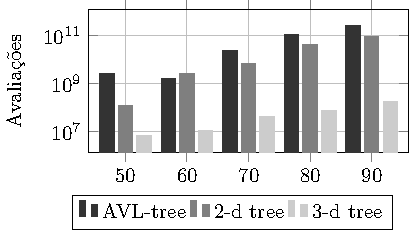
\includegraphics[scale=1.1]{tab/cmp/3dimA}
  \caption{Tipo A}
  \label{fig:sub5}
\end{subfigure}%
\begin{subfigure}{.5\textwidth}
  \centering
  %\begin{tikzpicture}
\begin{axis}[
	x tick label style={ /pgf/number format/1000 sep=},
	width=\cmpW, height=\cmpH,
	ylabel=Evaluations,
	ymode=log,
	grid = both,
	grid style={line width=.0pt, draw=gray!00},
	major grid style={line width=.2pt,draw=gray!50},
	%xlabel=Number of items (n),
	enlargelimits=0.15,
	legend style={at={(\legX,\legY)},
		anchor=north,legend columns=-1},
	ybar=2pt,% configures `bar shift'
	bar width=7pt,
	point meta=y *10^-7, % the displayed number
	cycle list = {black!80,black!50,black!20}
]

\addplot+[fill, text=black]
  coordinates {
    (100,2580591.4)
    (200,367842367.9)
    (300,7975491375.7)
    (400,72030125537.7)
  };

\addplot+[fill, text=black]
  coordinates {
    (100,1571248.6)
    (200,151476739.2)
    (300,2791493175.3)
    (400,45272872459.5)
  };
  
\addplot+[fill, text=black]
  coordinates {
    (100,912878.0)
    (200,29237583.4)
    (300,226471349.8)
    (400,960366212.0)
  };

\legend {AVL-tree,\dtree{2}, \dtree{3}}
\end{axis}
\end{tikzpicture}
  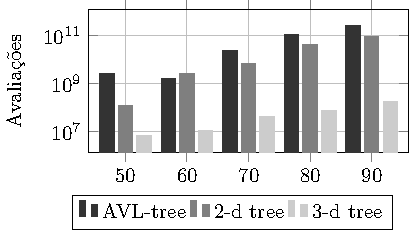
\includegraphics[scale=1.1]{tab/cmp/3dimA}
  \caption{Tipo B}
  \label{fig:sub6}
\end{subfigure}
\begin{subfigure}{.49\textwidth}
  \centering
  %\begin{tikzpicture}
\begin{axis}[
	x tick label style={ /pgf/number format/1000 sep=},
	width=\cmpW, height=\cmpH,
	ylabel=Avaliações,
	ymode=log,
	grid = both,
	grid style={line width=.1pt, draw=gray!00},
	major grid style={line width=.2pt,draw=gray!50},
	%xlabel=Number of items (n),
	enlargelimits=0.15,
	xtick={20, 30, 40},
	xticklabels={20, 30, 40},
	xmin=18,
	xmax=42,
	legend style={at={(\legX,\legY)},
		anchor=north,legend columns=-1},
	ybar=2pt,% configures `bar shift'
	bar width=7pt,
	point meta=y *10^-7, % the displayed number
	cycle list = {black!80,black!50,black!20}
]

\addplot+[fill, text=black]
  coordinates {
    ( 20,221956989)
    ( 30,10861341339)
    ( 40,26505319423)
  };

\addplot+[fill, text=black]
  coordinates {
    ( 20,235426288)
    ( 30,1340276850)
    ( 40,5943925097)
  };
  
\addplot+[fill, text=black]
  coordinates {
    ( 20,1919561)
    ( 30,10225751)
    ( 40,63529280)
  };

\legend {AVL-tree,\dtree{2}, \dtree{3}}
\end{axis}
\end{tikzpicture}

  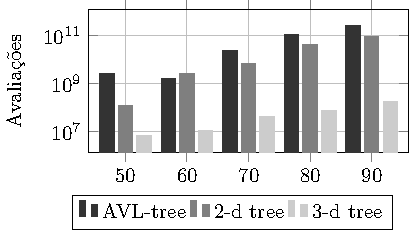
\includegraphics[scale=1.1]{tab/cmp/3dimA}
  \caption{Tipo C}
  \label{fig:sub7}
\end{subfigure}
\begin{subfigure}{.49\textwidth}
  \centering
  %\begin{tikzpicture}
\begin{axis}[
	x tick label style={ /pgf/number format/1000 sep=},
	width=\cmpW, height=\cmpH,
	ylabel=Evaluations,
	ymode=log,
	grid = both,
	grid style={line width=.0pt, draw=gray!00},
	major grid style={line width=.2pt,draw=gray!50},
	%xlabel=Number of items (n),
	enlargelimits=0.15,
	xtick={20, 30},
	xmin=17,
	xmax=33,
	legend style={at={(\legX,\legY)},
		anchor=north,legend columns=-1},
	ybar=2pt,% configures `bar shift'
	bar width=8pt,
	point meta=y *10^-7, % the displayed number
	cycle list = {black!80,black!50,black!20}
]

\addplot+[fill, text=black]
  coordinates {
    (20,481435295.3)
    (30,89269703684.8)
  };

\addplot+[fill, text=black]
  coordinates {
    (20,161607530.0)
    (30,32867842298.12)
  };
  
\addplot+[fill, text=black]
  coordinates {
    (20,2127432.7)
    (30,59136651.9)
  };

\legend {AVL-tree,\dtree{2}, \dtree{3}}
\end{axis}
\end{tikzpicture}
  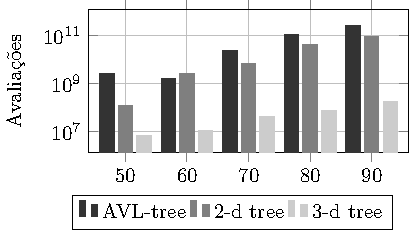
\includegraphics[scale=1.1]{tab/cmp/3dimA}
  \caption{Tipo D}
  \label{fig:sub8}
\end{subfigure}
